\documentclass[preprint, 3p,
authoryear]{elsarticle} %review=doublespace preprint=single 5p=2 column
%%% Begin My package additions %%%%%%%%%%%%%%%%%%%

\usepackage[hyphens]{url}

  \journal{Transportation Research Part A: Policy and
Practice} % Sets Journal name

\usepackage{lineno} % add

\usepackage{graphicx}
%%%%%%%%%%%%%%%% end my additions to header

\usepackage[T1]{fontenc}
\usepackage{lmodern}
\usepackage{amssymb,amsmath}
\usepackage{ifxetex,ifluatex}
\usepackage{fixltx2e} % provides \textsubscript
% use upquote if available, for straight quotes in verbatim environments
\IfFileExists{upquote.sty}{\usepackage{upquote}}{}
\ifnum 0\ifxetex 1\fi\ifluatex 1\fi=0 % if pdftex
  \usepackage[utf8]{inputenc}
\else % if luatex or xelatex
  \usepackage{fontspec}
  \ifxetex
    \usepackage{xltxtra,xunicode}
  \fi
  \defaultfontfeatures{Mapping=tex-text,Scale=MatchLowercase}
  \newcommand{\euro}{€}
\fi
% use microtype if available
\IfFileExists{microtype.sty}{\usepackage{microtype}}{}
\usepackage[]{natbib}
\bibliographystyle{plainnat}

\ifxetex
  \usepackage[setpagesize=false, % page size defined by xetex
              unicode=false, % unicode breaks when used with xetex
              xetex]{hyperref}
\else
  \usepackage[unicode=true]{hyperref}
\fi
\hypersetup{breaklinks=true,
            bookmarks=true,
            pdfauthor={},
            pdftitle={How is active school travel framed in Ontario, Canada?},
            colorlinks=false,
            urlcolor=blue,
            linkcolor=magenta,
            pdfborder={0 0 0}}

\setcounter{secnumdepth}{5}
% Pandoc toggle for numbering sections (defaults to be off)


% tightlist command for lists without linebreak
\providecommand{\tightlist}{%
  \setlength{\itemsep}{0pt}\setlength{\parskip}{0pt}}



\usepackage{booktabs}
\usepackage{longtable}
\usepackage{array}
\usepackage{multirow}
\usepackage{wrapfig}
\usepackage{float}
\usepackage{colortbl}
\usepackage{pdflscape}
\usepackage{tabu}
\usepackage{threeparttable}
\usepackage{threeparttablex}
\usepackage[normalem]{ulem}
\usepackage{makecell}
\usepackage{xcolor}



\begin{document}


\begin{frontmatter}

  \title{How is active school travel framed in Ontario, Canada?}
    \author[McMaster University]{Elise Desjardins%
  %
  }
   \ead{desjae@mcmaster.ca} 
    \author[McMaster University]{Jason Lam%
  %
  }
   \ead{lamj54@mcmaster.ca} 
    \author[University of Alberta]{Darcy Reynard%
  %
  }
   \ead{reynard@ualberta.ca} 
    \author[University of Alberta]{Damian Collins%
  %
  }
   \ead{damian.collins@ualberta.ca} 
    \author[Polytechnique Montreal]{E. Owen D. Waygood%
  %
  }
   \ead{owen.waygood@polymtl.ca} 
    \author[McMaster University]{Antonio Paez%
  \corref{cor1}%
  \fnref{1}}
   \ead{paezha@mcmaster.ca} 
      \affiliation[McMaster University]{School of Earth, Environment and
Society, 1280 Main St.~W, Hamilton, Ontario, Canada L8S 4K1}
    \affiliation[University of Alberta]{Department of Earth and
Atmospheric Sciences, 1-26 Earth Sciences Building, Edmonton, Alberta,
Canada T6G 2E3}
    \affiliation[Polytechnique Montreal]{Department of Civil, Geological
and Mining Engineering, 2500, chemin de Polytechnique Montreal,
Montreal, Quebec, Canada H3T 1J4}
    \cortext[cor1]{Corresponding author}
    \fntext[1]{Corresponding author.}
  
  \begin{abstract}
  Active school travel (AST) has been increasingly encouraged by various
  stakeholders in Ontario, Canada through efforts such as school travel
  planning. Education strategies like workshops or resources that
  promote AST are commonly implemented. The framing of AST through such
  strategies may influence how walking and bicycling to school are
  perceived by parents. It may also draw attention to AST as an issue
  affecting children's health which could motivate behaviour change. We
  used natural language processing, including topic modelling, to
  examine how AST is framed in publicly available documents from Ontario
  stakeholders involved in school travel planning. We then compared the
  findings from these documents to a selection of studies on AST and
  explored similarities between the two. We found that AST is framed in
  two ways: i) as a health and environmental issue; and ii) as an
  accessible and feasible transport option for children and parents. The
  frames encourage children and parents to adopt AST given its health
  and environmental benefits by providing resources to support behaviour
  change. The benefits of AST and strategies to support AST that are
  communicated by stakeholders are consistent with the evidence from
  academic research. While these frames present AST in a positive light,
  they may not encourage parents to view current household travel
  behaviours as unhealthy for their children or their community.
  Stakeholders promoting AST in Ontario should further problematize the
  decline of AST and challenge the norm of driving children to school.
  \end{abstract}
    \begin{keyword}
    active school travel \sep school travel planning \sep natural
language processing \sep 
    framing analysis
  \end{keyword}
  
 \end{frontmatter}

\newpage

\hypertarget{introduction}{%
\section{Introduction}\label{introduction}}

Walking and bicycling to school, commonly known as active school travel
(AST), have declined in North America for decades
\citep{rothmanDeclineActiveSchool2018}, but the appetite for these modes
is beginning to rise in many Canadian communities. For instance,
research in Toronto, Ontario found that 40\% of children who were driven
to school would like to travel by bicycle instead
\citep{laroucheRatherBikeSchool2016}. Another study in London, Ontario,
reported similar findings with respect to children's preference for
active travel \citep{larsenRouteBasedAnalysisCapture2012}. From a public
health perspective, increasing active travel to school represents a
major opportunity to improve children's health and wellbeing.

To promote this trend, in 2017 the Government of Ontario began to
support communities develop AST initiatives through a program called
\emph{Ontario Active School Travel} (OAST). By 2021, the program, run by
Green Communities Canada had awarded over CAD 2 million and provided
resources to over 25 projects across Ontario
\citep{GreenCommunities2016}. A popular intervention in many communities
is school travel planning (STP) \citep[see][]{GreenCommunitiesProjects}.
In this context, STPs are ``school-specific'' interventions led by a
facilitator who works with a committee of stakeholders from diverse
sectors including education, planning, transportation, and public health
to develop action plans
\citep{buliungSchoolTravelPlanning2011, mammenSchoolTravelPlanning2014}.
The five-step process involves identifying barriers to AST and
implementing solutions or activities to make AST safer and more
convenient: 1) setup of the program; 2) data collection and problem
identification; 3) action planning; 4) implementation; 5) monitoring and
evaluation
\citep{buliungSchoolTravelPlanning2011, langUnderstandingModalChoice2011}.

Framing AST by STP stakeholders to a target audience (e.g., parents or
the general public) can raise awareness of the relevant issues and
influence how active travel to school is perceived. Gamson and
Modigliani \citeyearpar{gamsonChangingCulture1987} define a frame as a
``central organizing idea or story line that provides meaning'' to a
particular phenomenon. A frame can enable individuals ``to locate,
perceive, identify, and label'' information pertaining to various
dimensions of an issue \citep{goffmanFrameAnalysisEssay1974}. Therefore,
stakeholders involved in STP efforts can play a role in shaping public
perception about AST to attract greater attention and recognition as a
``problem'' that needs to be addressed through behaviour change or new
policies.

After significant investment of human and financial resources to boost
rates of AST in Ontario over the past few years, in this paper we ask
this central question: How is AST framed to the public in Ontario? The
following questions are subsidiary and help us address this main
question: What benefits of AST are communicated to the public? What
solutions are proposed to increase AST?

We approach this question by means of natural language processing, and
examine how three STP stakeholder groups in Ontario (municipalities,
school boards, and transportation consortia) frame AST. We assemble a
corpus of texts from public sources that present information for the
general public or parents who are interested in AST. We examine word
frequency, bigrams, and concordances in these selected documents, and
also identify key topics presented by each stakeholder group. We then
compare the findings from these documents to a selection of studies on
AST and explore the extent to which there is concordance between the
scholarly literature on AST and materials shared with the public.

\hypertarget{literature-review-ast}{%
\section{Literature Review: AST}\label{literature-review-ast}}

The desire to increase AST in Canada is warranted given its potential
physical and mental health benefits. Faulkner et al.
\citeyearpar{faulknerActiveSchoolTransport2009} concluded from their
systematic review that children who travel on foot or by bicycle to
school generally have higher levels of physical activity than their
peers who are driven to school. This relationship could be
dose-dependent, and contingent on sufficiently long trips to school to
accumulate physical activity. A walking distance of 1000-1600 metres to
school has been found to contribute to overall levels of physical
activity for boys \citep{faulknerSchoolTravelChildren2013}. The daily
routine of travelling to school can be a good opportunity for children
to regularly build physical activity into their schedule
\citep{mitraIndependentMobilityMode2013}.

More recently, the link between transport and children's wellbeing has
attracted interest too \citep{waygoodTransportChildrenWellbeing2020}.
Being driven to school reduces community interactions for children,
which may negatively impact their social wellbeing
\citep{waygoodChildrenTravelIncidental2015}. In contrast, walking and
bicycling give children opportunities to socialize
\citep{michailChildrenExperiencesTheir2021} and increase positive
emotions that contribute to wellbeing
\citep{ramanathanHappinessMotionEmotions2014a}, a feeling that children
seem to value \citep{zwertsHowChildrenView2010}. AST can also provide
opportunities for children to engage with natural environments
\citep{fuscoUnderstandingChildrenPerceptions2012, romeroChildrenExperiencesEnjoyment2015}.

Factors that influence AST have been presented and organized using a
socio-ecological model (SEM) \citep{mitraIndependentMobilityMode2013} or
systems model \citep{badlandDevelopmentSystemsModel2016} whereby
children's travel behaviour is understood within the context of
household, social, neighbourhood, and policy environments. The SEM helps
to identify multiple determinants that need to be addressed by
school-based interventions to increase AST, with the consensus being
that interventions should target multiple levels
\citep{mitraIndependentMobilityMode2013}. Rather than describing an
extensive list of factors that influence AST and mode choice in Canada
\citep[e.g.,][]{mammenUnderstandingDriveEscort2012, mitraIndependentMobilityMode2013, rothmanDeclineActiveSchool2018, wilsonUnderstandingChildParent2018},
we discuss a few potentially modifiable determinants that may be
targeted for change through STP.

Children's mode choice to school is strongly influenced by their
parents' travel behaviours and the complexity of their household's
travel needs \citep{buliungLivingJourneySchool2021}, as well as daily
parental support \citep{mahDoesParentalSupport2017a}. This indicates
that shifting parental perceptions and habits is important. Convenience
and inclement weather have been cited by parents as barriers to AST
\citep{buliungSchoolTravelPlanning2011}. Parental perceptions of the
built or school environment
\citep{demeesterParentalPerceivedNeighborhood2014, panterAttitudesSocialSupport2010}
and their children's skills
\citep{mammenUnderstandingDriveEscort2012, faulknerWhatQuickestEasiest2010}
also influence mode choice to school.

Distance between home and school is most negatively associated with AST
\citep{ikedaAssociationsChildrenActive2018, mammenUnderstandingDriveEscort2012, pontEnvironmentalCorrelatesChildren2009, rothmanDeclineActiveSchool2018}
with less AST reported among children who have to travel farther to
school. Many studies have also found that the quality of the built
environment along the route to school and around the school site
\citep{ikedaAssociationsChildrenActive2018, rothmanActiveSchoolTransportation2021}
and provision of active travel infrastructure
\citep{chenPromotingActiveStudent2018, pontEnvironmentalCorrelatesChildren2009}
facilitate AST. Canadian youth report that they feel most safe bicycling
on streets in their neighbourhood or that have low volumes of traffic
\citep{TACbikeinfra2020}. Finally, concerns about traffic and strangers
have been reported by parents who drive their children to school
\citep{mammenUnderstandingDriveEscort2012}, which highlights that the
volume and speed of cars can be a concern or deterrent for AST.

\hypertarget{school-travel-planning-in-canada-and-relevance-of-framing-analysis}{%
\section{School travel planning in Canada and relevance of framing
analysis}\label{school-travel-planning-in-canada-and-relevance-of-framing-analysis}}

School travel planning (STP) has been implemented in Canada since at
least the late 2000s. Within the STP process, facilitators establish
multi-sector committees which intervene at the participating school
through a range of activities consisting of \emph{{[}E{]}ducation}
strategies, \emph{{[}E{]}ncouragement} through in-person events or
programs, \emph{{[}E{]}ngineering} improvements to or around the school
site, and \emph{{[}E{]}nforcement} of traffic speeds around schools
\citep[or
4Es,][]{langUnderstandingModalChoice2011, mammenActiveSchoolTravel2014}.
Following the first large-scale evaluation of STP as an intervention in
Canada, AST rates increased and 14\% of parents reported a perceived
reduction in traffic outside the school
\citep{buliungSchoolTravelPlanning2011}. Assessments of the efficacy of
STP
\citep{buttazzoniPromotingActiveSchool2019, mammenActiveSchoolTravel2014}
indicate its potential to encourage behaviour change and adoption of
AST.

By providing a ``central organizing idea or story line''
\citep{gamsonChangingCulture1987} framing of AST seems particularly
important to shift parental attitudes and perceptions, given their
reported influence on children's travel mode to school. Scholars in the
field of political communications have proposed that communicators, such
as the media or institutions, construct the narrative of a frame for
policy positions or public issues in order to activate or restrict a
particular response in the intended audience
\citep{panFramingAnalysisApproach1993}. Organized groups of stakeholders
can employ similar methods to attract attention to particular issues.
Framing can be used to position existing solutions as suitable to
address particular issues \citep{mahFramecriticalPolicyAnalysis2014},
which may prevent the public from being aware of other policy approaches
that challenge the status quo. The way policy issues are framed is
ultimately important to understand because it plays a role in either
altering or preserving the existing social perceptions. Finally, the
ideas that are communicated by a particular frame can be either positive
or negative \citep{waygoodCO2ValenceFraming2018}. There is evidence that
negative framing may be more effective at motivating individuals, for
example, to change transport modes to reduce CO2 emissions
\citep{waygoodCO2ValenceFraming2018}.

Framing of AST could also affect broader support in the community.
Municipal representatives are perceived to be instrumental but the
involvement of other stakeholder groups (e.g., busing consortia
representatives and local residents) can be lacking
\citep{buttazzoniSupportingActiveSchool2018}. In Ontario, it is
reasonable to say that AST has become a policy issue on the education
and public health agendas, supported, albeit in a modest way, by
financial contributions from the provincial government. Still, the
support from a range of municipal representatives
\citep[see][]{buttazzoniSupportingActiveSchool2018, mammenPuttingSchoolTravel2015}
demonstrates that the AST issue is on the political agenda.

Since STP activities heavily focus on education or encouragement
\citep{buliungSchoolTravelPlanning2011, mammenActiveSchoolTravel2014, buttazzoniSupportingActiveSchool2018},
it is important that parents and communities are receptive to the goals
of STP \citep{buttazzoniSupportingActiveSchool2018}. Parents have been
found to express different understandings, language, and perceptions
than planners of how the built environment can influence school travel
\citep{buliungLivingJourneySchool2021}. This is also true when it comes
to other factors like convenience of different modes to school
\citep{langUnderstandingModalChoice2011}. STP stakeholders must pay
special attention to parents' understanding of the decline of AST as a
problem, which may affect their receptivity to proposed solutions.

The success of STP interventions would likely depend on parental
judgments of factors that are related to school travel, as well as
support from key policy makers. For example, parents have been found to
view mixed land use as conducive for driving, despite transport planners
viewing neighbourhoods with mixed uses as key for encouraging more
active travel \citep{buliungLivingJourneySchool2021}. Therefore,
stakeholders involved in STP must make conscious choices about the
proposed solutions and potential benefits of AST that are communicated
to parents and the general public through publicly available content to
convey its importance as a policy issue and to facilitate adoption of
AST.

\hypertarget{data}{%
\section{Data}\label{data}}

\hypertarget{data-retrieval}{%
\subsection{Data retrieval}\label{data-retrieval}}

\hypertarget{policy-documents}{%
\subsubsection{Policy documents}\label{policy-documents}}

We assembled a collection of publicly available documents that were
sourced online from the main stakeholder groups involved in STP
initiatives in Ontario: i) school boards (public or Catholic and
English-speaking only); ii) municipal governments; and iii)
transportation consortia. The latter involve a collaboration between
municipal regions and school boards to deliver more efficient and timely
transportation services to schools in each region. Non-profit
organizations, police services, and advocacy groups are other
stakeholders who often play a role in supporting AST and/or STP, but
this study does not include any documents from these groups because they
do not consistently participate in STP initiatives in Ontario.

The search was guided first by a list of all English public and Catholic
school boards across Ontario. The websites of each school board were
manually searched for pages related to school transport or travel. Any
pages relevant to these topics were downloaded. Next, we searched
municipal government and transportation consortia websites. These were
identified based on geographic area. Likewise, webpages related to
active transport or school travel were downloaded.

Webpages from STP stakeholder groups were included in our analysis if
they were findable. This primary criterion was important since our
analysis pertains to how such issues are framed to the general public.
Thus, we included only webpages that were readily accessible, which we
defined as requiring no more than four links from the initial Google
search to reach.

The initial corpus of documents from STP stakeholder groups included 69
relevant webpages. We refer to these as policy+practice documents
throughout the paper. It is important to note that school boards,
municipalities, and transportation consortia may or may not publish
information about their involvement in AST and STP efforts on their
respective websites or in policy documents. Search results are
summarized in Table \ref{tab:policy-documents}.

\begin{table}

\caption{\label{tab:policy-documents}\label{tab:search-results}Search results from the main STP stakeholder groups.}
\centering
\begin{tabular}[t]{>{}l|l|>{}l}
\toprule
Stakeholder & Total & Retrieved\\
\midrule
\cellcolor{gray!6}{\textbf{School boards}} & \cellcolor{gray!6}{62} & \cellcolor{gray!6}{32}\\
\textbf{Municipalities} & 62 & 28\\
\cellcolor{gray!6}{\textbf{Transportation consortia}} & \cellcolor{gray!6}{39} & \cellcolor{gray!6}{9}\\
\bottomrule
\end{tabular}
\end{table}

\hypertarget{academic-papers}{%
\subsubsection{Academic papers}\label{academic-papers}}

We conducted a search on Web of Science for scholarly papers on the
topic of school travel. We limited our search to the fields of public
health, transportation, planning, urban studies, and geography. This
initial corpus was curated by the authors to ensure that all documents
were relevant. After this step, 227 journal articles were readied for
analysis.

\hypertarget{data-cleaning}{%
\subsection{Data cleaning}\label{data-cleaning}}

A multi-step process was conducted to ensure that the analysis captured
as much text as possible from both the policy documents (n = 64) and
academic papers (n = 227). Webpages were manually downloaded in portable
document format (PDF) and trimmed so that pages that only consisted of
tables, figures, or references were removed. After converting into
\texttt{txt} files and importing for analysis, we manually removed any
remaining tables, figures, references, headers/footings, and captions
that could not be trimmed. We also manually removed any extraneous
material that did not pertain to AST specifically (e.g., references,
footnotes, weblinks, etc.). In the final step, we removed all blank
spaces, punctuation, capitalization, and numbers. English stop words
(i.e., words such as \emph{and} or \emph{the}) and other frequent terms
in the documents like ``school'' and specific location names were
removed from the corpora.

\hypertarget{methods}{%
\section{Methods}\label{methods}}

\hypertarget{process-of-framing-analysis}{%
\subsection{Process of Framing
Analysis}\label{process-of-framing-analysis}}

We use topic modelling to analyze the documents retrieved. Topic
modelling is a natural language processing technique used to analyze
text to identify the language and concepts being communicated. This
method is practical for researchers working with large amounts of text
because it replaces the manual coding of topics that would normally take
place to analyze or summarize textual data
\citep{jacobiQuantitativeAnalysisLarge2016}. We primarily use the
following software: \texttt{tidytext} \citep{R-tidytext},
\texttt{topicmodels} \citep{R-topicmodels}, \texttt{word2vec}
\citep{R-word2vec}, and \texttt{wordcloud} \citep{R-wordcloud}.

We estimate latent Dirichlet allocation (LDA) models to identify topics
contained in both the STP and academic documents. The model's output is
``a set of topics consisting of clusters of words that co-occur in these
documents according to certain patterns''
\citep{jacobiQuantitativeAnalysisLarge2016}. Researchers must then
interpret the identified topics, as done after other methods of manual
coding.

\hypertarget{reproducibility}{%
\subsection{Reproducibility}\label{reproducibility}}

This paper is an example of open and reproducible research that uses
only open software. Following best practices in spatial data science
\citep{brunsdon2020opening}, the code and data needed to reproduce our
research or conduct a similar analysis for other regions are available
for download upon request.

\hypertarget{results}{%
\section{Results}\label{results}}

\hypertarget{word-and-document-frequency}{%
\subsection{Word and document
frequency}\label{word-and-document-frequency}}

We analyzed word and document frequency for each corpus of text. Table
\ref{tab:word-table} shows the most frequent terms found in the
municipal, transportation consortia, school board, and academic
documents. Policy documents and academic papers reference \emph{active},
\emph{travel}, \emph{walking}, \emph{biking} or \emph{cycling}, and
\emph{students} more than other terms. Each corpus also has
\emph{safety} and \emph{traffic} as common words which suggests that
these are common concerns for parents. The word \emph{physical} is
present in each corpus, but it's not clear what this refers to (e.g,
\emph{physical activity}, or the \emph{physical environment}).
Furthermore, documents from STP stakeholder groups discuss
\emph{resources}, \emph{information}, and \emph{services} about school
travel. Unlike the academic papers, policy+practice documents include
the words \emph{route} or \emph{routes} as frequent terms. This could
indicate the role of STP stakeholder groups in identifying safe routes
to school to share with parents or families. In the section below, the
context in which these terms are used is explored further.

The academic corpus differs from the policy documents in that
\emph{parents} and \emph{distance} are the second and third most common
terms. In addition, \emph{time}, \emph{factors}, \emph{environment}, and
\emph{age} are also identified in the academic papers. The prevalence of
these terms is consistent with an academic focus on exploring the
variables that influence mode choice. These words are absent from the
list of common words in policy+practice documents. Table
\ref{tab:word-table} indicates that the academic corpus discusses a
broader range of determinants of AST than the policy documents. The
number of references for each term in the academic papers is also
substantially higher due to the inclusion of more documents.

\begin{table}

\caption{\label{tab:word-table}\label{tab:word-table}Top 25 terms identified in each corpus. Document frequencies are also indicated.}
\centering
\resizebox{\linewidth}{!}{
\begin{tabular}[t]{lcclcclcclcc}
\toprule
\multicolumn{3}{c}{Municipalities} & \multicolumn{3}{c}{School Boards} & \multicolumn{3}{c}{Transportation Consortia} & \multicolumn{3}{c}{Academic Papers} \\
\cmidrule(l{3pt}r{3pt}){1-3} \cmidrule(l{3pt}r{3pt}){4-6} \cmidrule(l{3pt}r{3pt}){7-9} \cmidrule(l{3pt}r{3pt}){10-12}
Term & Count (n) & Documents (n) & Term & Count (n) & Documents (n) & Term & Count (n) & Documents (n) & Term & Count (n) & Documents (n)\\
\midrule
\cellcolor{gray!6}{active} & \cellcolor{gray!6}{248} & \cellcolor{gray!6}{26} & \cellcolor{gray!6}{active} & \cellcolor{gray!6}{124} & \cellcolor{gray!6}{13} & \cellcolor{gray!6}{active} & \cellcolor{gray!6}{67} & \cellcolor{gray!6}{7} & \cellcolor{gray!6}{walking} & \cellcolor{gray!6}{5059} & \cellcolor{gray!6}{220}\\
travel & 126 & 20 & bus & 120 & 20 & walking & 55 & 8 & parents & 3927 & 209\\
\cellcolor{gray!6}{walking} & \cellcolor{gray!6}{90} & \cellcolor{gray!6}{25} & \cellcolor{gray!6}{travel} & \cellcolor{gray!6}{103} & \cellcolor{gray!6}{11} & \cellcolor{gray!6}{walk} & \cellcolor{gray!6}{49} & \cellcolor{gray!6}{8} & \cellcolor{gray!6}{distance} & \cellcolor{gray!6}{3252} & \cellcolor{gray!6}{203}\\
bike & 87 & 15 & information & 65 & 21 & travel & 41 & 8 & students & 2956 & 171\\
\cellcolor{gray!6}{cycling} & \cellcolor{gray!6}{78} & \cellcolor{gray!6}{22} & \cellcolor{gray!6}{walking} & \cellcolor{gray!6}{57} & \cellcolor{gray!6}{17} & \cellcolor{gray!6}{students} & \cellcolor{gray!6}{39} & \cellcolor{gray!6}{9} & \cellcolor{gray!6}{cycling} & \cellcolor{gray!6}{2739} & \cellcolor{gray!6}{170}\\
\addlinespace
safety & 71 & 21 & walk & 53 & 13 & safety & 32 & 6 & environment & 2585 & 200\\
\cellcolor{gray!6}{health} & \cellcolor{gray!6}{65} & \cellcolor{gray!6}{21} & \cellcolor{gray!6}{weather} & \cellcolor{gray!6}{40} & \cellcolor{gray!6}{11} & \cellcolor{gray!6}{help} & \cellcolor{gray!6}{29} & \cellcolor{gray!6}{9} & \cellcolor{gray!6}{traffic} & \cellcolor{gray!6}{2334} & \cellcolor{gray!6}{206}\\
physical & 63 & 18 & safety & 40 & 19 & schools & 25 & 9 & choice & 2295 & 167\\
\cellcolor{gray!6}{traffic} & \cellcolor{gray!6}{59} & \cellcolor{gray!6}{20} & \cellcolor{gray!6}{safe} & \cellcolor{gray!6}{39} & \cellcolor{gray!6}{19} & \cellcolor{gray!6}{children} & \cellcolor{gray!6}{25} & \cellcolor{gray!6}{6} & \cellcolor{gray!6}{activity} & \cellcolor{gray!6}{2265} & \cellcolor{gray!6}{207}\\
road & 56 & 13 & services & 37 & 17 & community & 24 & 7 & physical & 2238 & 213\\
\addlinespace
\cellcolor{gray!6}{activity} & \cellcolor{gray!6}{55} & \cellcolor{gray!6}{14} & \cellcolor{gray!6}{planning} & \cellcolor{gray!6}{37} & \cellcolor{gray!6}{7} & \cellcolor{gray!6}{bus} & \cellcolor{gray!6}{18} & \cellcolor{gray!6}{4} & \cellcolor{gray!6}{trips} & \cellcolor{gray!6}{2164} & \cellcolor{gray!6}{168}\\
schools & 52 & 14 & parents & 32 & 17 & route & 17 & 5 & car & 2140 & 193\\
\cellcolor{gray!6}{children} & \cellcolor{gray!6}{47} & \cellcolor{gray!6}{15} & \cellcolor{gray!6}{sustainable} & \cellcolor{gray!6}{31} & \cellcolor{gray!6}{8} & \cellcolor{gray!6}{zone} & \cellcolor{gray!6}{16} & \cellcolor{gray!6}{6} & \cellcolor{gray!6}{safety} & \cellcolor{gray!6}{2111} & \cellcolor{gray!6}{202}\\
plan & 45 & 16 & children & 31 & 14 & resources & 16 & 6 & time & 2091 & 216\\
\cellcolor{gray!6}{students} & \cellcolor{gray!6}{44} & \cellcolor{gray!6}{14} & \cellcolor{gray!6}{child} & \cellcolor{gray!6}{31} & \cellcolor{gray!6}{12} & \cellcolor{gray!6}{day} & \cellcolor{gray!6}{16} & \cellcolor{gray!6}{4} & \cellcolor{gray!6}{factors} & \cellcolor{gray!6}{2083} & \cellcolor{gray!6}{214}\\
\addlinespace
walk & 43 & 18 & day & 29 & 13 & safe & 15 & 5 & child & 2060 & 185\\
\cellcolor{gray!6}{public} & \cellcolor{gray!6}{39} & \cellcolor{gray!6}{15} & \cellcolor{gray!6}{routes} & \cellcolor{gray!6}{28} & \cellcolor{gray!6}{14} & \cellcolor{gray!6}{planning} & \cellcolor{gray!6}{15} & \cellcolor{gray!6}{4} & \cellcolor{gray!6}{walk} & \cellcolor{gray!6}{1985} & \cellcolor{gray!6}{198}\\
community & 37 & 19 & physical & 28 & 11 & physical & 15 & 7 & public & 1973 & 206\\
\cellcolor{gray!6}{safe} & \cellcolor{gray!6}{34} & \cellcolor{gray!6}{16} & \cellcolor{gray!6}{health} & \cellcolor{gray!6}{28} & \cellcolor{gray!6}{11} & \cellcolor{gray!6}{healthy} & \cellcolor{gray!6}{14} & \cellcolor{gray!6}{6} & \cellcolor{gray!6}{age} & \cellcolor{gray!6}{1774} & \cellcolor{gray!6}{209}\\
benefits & 32 & 17 & inclement & 25 & 11 & traffic & 13 & 6 & urban & 1749 & 198\\
\addlinespace
\cellcolor{gray!6}{play} & \cellcolor{gray!6}{31} & \cellcolor{gray!6}{2} & \cellcolor{gray!6}{eligibility} & \cellcolor{gray!6}{24} & \cellcolor{gray!6}{11} & \cellcolor{gray!6}{support} & \cellcolor{gray!6}{13} & \cellcolor{gray!6}{6} & \cellcolor{gray!6}{different} & \cellcolor{gray!6}{1695} & \cellcolor{gray!6}{213}\\
resources & 30 & 13 & consortium & 24 & 9 & families & 13 & 5 & home & 1691 & 197\\
\cellcolor{gray!6}{healthy} & \cellcolor{gray!6}{29} & \cellcolor{gray!6}{16} & \cellcolor{gray!6}{region} & \cellcolor{gray!6}{23} & \cellcolor{gray!6}{10} & \cellcolor{gray!6}{way} & \cellcolor{gray!6}{12} & \cellcolor{gray!6}{5} & \cellcolor{gray!6}{social} & \cellcolor{gray!6}{1672} & \cellcolor{gray!6}{189}\\
routes & 27 & 13 & service & 22 & 11 & student & 12 & 5 & significant & 1644 & 206\\
\cellcolor{gray!6}{lanes} & \cellcolor{gray!6}{26} & \cellcolor{gray!6}{3} & \cellcolor{gray!6}{•} & \cellcolor{gray!6}{21} & \cellcolor{gray!6}{1} & \cellcolor{gray!6}{region} & \cellcolor{gray!6}{12} & \cellcolor{gray!6}{4} & \cellcolor{gray!6}{mobility} & \cellcolor{gray!6}{1634} & \cellcolor{gray!6}{136}\\
\bottomrule
\multicolumn{12}{l}{\rule{0pt}{1em}\textit{Note: }}\\
\multicolumn{12}{l}{\rule{0pt}{1em} }\\
\multicolumn{12}{l}{\rule{0pt}{1em}\textsuperscript{a} Count (n) refers to the total number of times the term is found in the corpora}\\
\multicolumn{12}{l}{\rule{0pt}{1em}\textsuperscript{b} Documents (n) refers to the total number of documents that feature the term}\\
\end{tabular}}
\end{table}

Examination of document frequency reveals terms that are not present in
all policy documents. This suggests that although documents pertain to
the subject of school travel, not all stakeholders across Ontario
disseminate information about AST. We manually searched the
policy+practice corpus and found that 48\% of documents mention AST and
16\% mention STP. In contrast, inclement weather and its impacts on
busing is a common topic addressed in school board and transportation
consortia documents.

\hypertarget{bigrams-and-concordances}{%
\subsection{Bigrams and concordances}\label{bigrams-and-concordances}}

\begin{figure}

{\centering 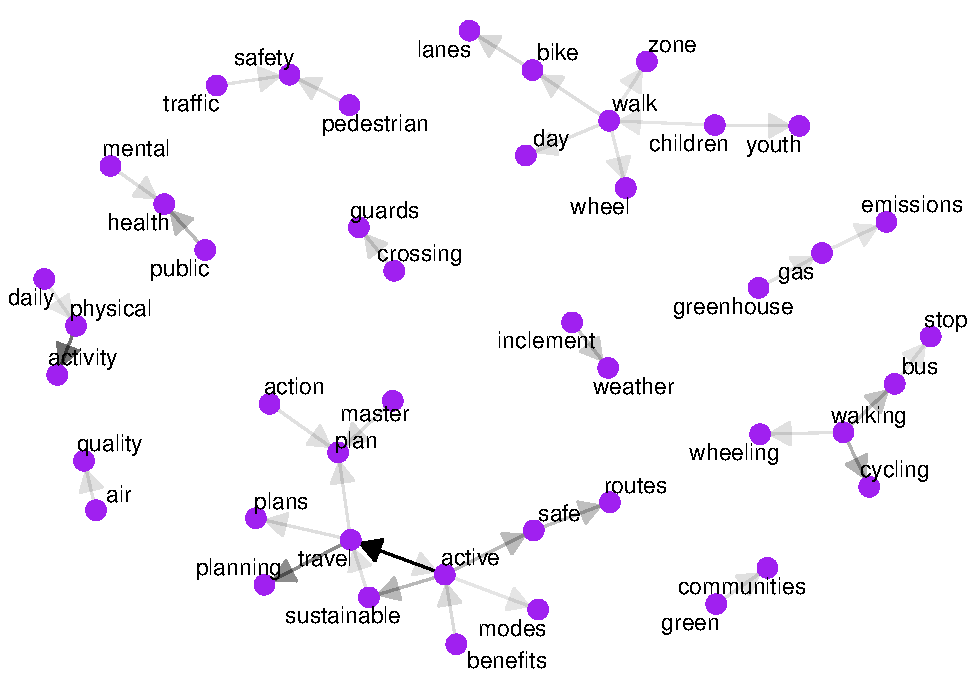
\includegraphics[width=1\linewidth]{AST-Framing-Ontario_files/figure-latex/policy-visual-1} 

}

\caption{\label{fig:policy-visual}Most common bigrams found across all policy documents (i.e., school board, municipality, and transportation consortia combined).}\label{fig:policy-visual}
\end{figure}

Bigrams refer to a pair of consecutive words. We combined all
municipality, school board, and transportation consortia documents into
the policy+practice. Figure \ref{fig:policy-visual} shows all of the
bigrams that occur more than 10 times in the policy+practice corpus.
This figure highlights the main ideas that are presented to the public
in each of the policy corpora. The directional arrows indicate the
arrangement of the words (e.g., active travel and not travel active) and
the colour gradient of the arrows corresponds to the most frequently
mentioned pairs (e.g., bigrams with darker arrows are found in the
corpus more often).

STP stakeholders discuss \emph{physical activity} and \emph{public
health} in the context of AST. In addition, \emph{travel planning},
\emph{bike lanes}, and \emph{safe routes} are also identified,
conceivably as either proposed solutions or built environment factors
that support AST. Key issues related to transport such as \emph{traffic
safety}, \emph{air quality}, and \emph{greenhouse gases} are conveyed to
the public through these policy documents. It is not surprising to find
this focus given that municipalities in Ontario are concerned about
climate change and have increasingly looked to active travel to offset
transport-related emissions in urban areas. We also found \emph{mental
health}, \emph{walk zone}, and \emph{green communities} as common pairs
of consecutive words. \emph{Green Communities Canada} is a non-profit
organization that has significantly supported AST initiatives through
the Ontario Active School Travel program so the high frequency of this
term in the policy+practice corpus is not surprising. Overall, the
policy documents from STP stakeholder groups seem to focus on four key
areas: i) benefits or impacts of AST; ii) mechanisms of intervention;
iii) concerns or barriers; and iv) supports for AST. This interpretation
indicates that the general public accessing information about AST in
Ontario is informed about a wide range of content related to this issue.

Next, we analyzed bigrams in the academic corpus separately to make
comparisons with the policy+practice corpus. Figure
\ref{fig:academic-visual} indicates that academic papers include several
common bigrams that were also found in the policy documents including
\emph{physical activity}, which is the top bigram, \emph{traffic
safety}, and \emph{safe routes}. However, many other factors are
identified in the research literature that are not presented to the
general public through policy documents. Terms like \emph{built
environment}, \emph{independent mobility}, and \emph{urban form} are
other frequent pairs of consecutive words. Academic papers also often
discuss \emph{distance home}, \emph{car ownership}, \emph{household
income}, and \emph{population density}, which are factors that have been
found to influence AST. Finally, the presence of \emph{statistically
significant} among the top bigrams indicates that researchers often aim
to identify associations using statistical measures. We found that the
academic corpus focuses on a greater range of topics than found in the
policy+practice documents.

\begin{figure}

{\centering 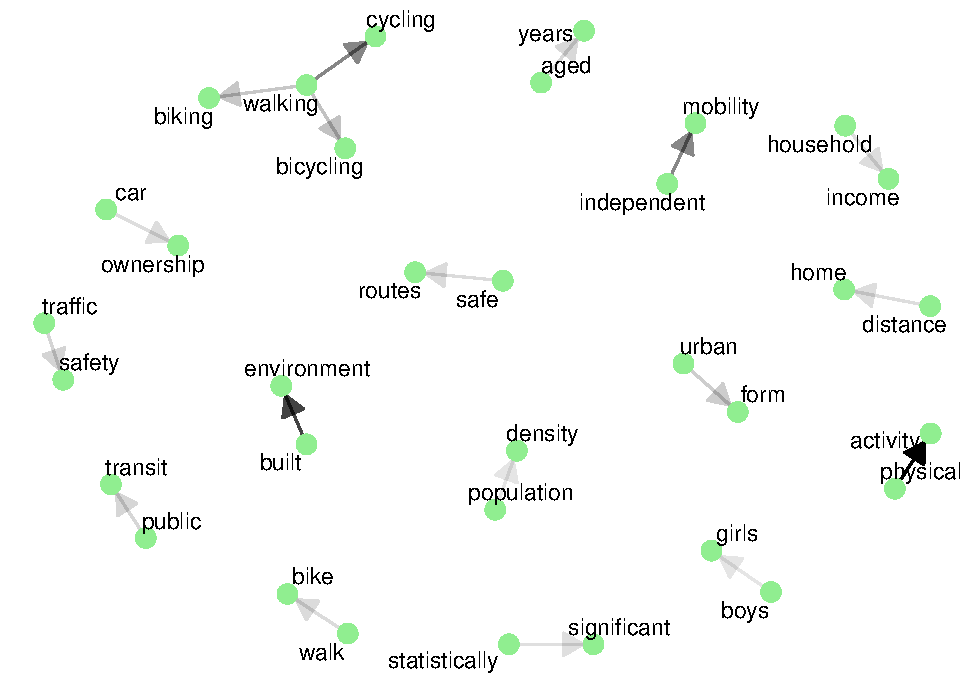
\includegraphics[width=1\linewidth]{AST-Framing-Ontario_files/figure-latex/academic-visual-1} 

}

\caption{\label{fig:academic-visual}Most common bigrams found in the academic papers.}\label{fig:academic-visual}
\end{figure}

We interpreted the most common bigrams from the policy+practice corpus
(see Figure \ref{fig:policy-visual}) as the main ideas that STP
stakeholder groups focus on and communicate to the public about AST. We
then examined the context of these key ideas by extracting
words-in-context from the corpora. Table \ref{tab:policy-concordance}
presents some examples from select policy documents that illustrate how
the most common bigrams are communicated to the public.

\begin{table}

\caption{\label{tab:content-table}\label{tab:policy-concordance}The context of key terms that were identified as common bigrams.}
\centering
\begin{tabular}[t]{>{}ll>{\raggedright\arraybackslash}p{20em}}
\toprule
Terms & Stakeholder & Context\\
\midrule
\textbf{\cellcolor{gray!6}{Air Quality}} & \cellcolor{gray!6}{School Board} & \cellcolor{gray!6}{Active transportation [...] improves air quality.}\\
\textbf{Benefit} & Municipality & Stronger bones and muscles, improved self-esteem and sense of well-being while reducing stress and risk of chronic disease all benefit those who use active transportation.\\
\textbf{\cellcolor{gray!6}{Walking School Bus}} & \cellcolor{gray!6}{School Board} & \cellcolor{gray!6}{While taking part in a walking school bus, your child will enjoy seeing friends on the way to school. They will be active more often. This is also a great opportunity for your child to socialize with school friends in a monitored and safe way where they can practice social distancing, modelled by a leader.}\\
\textbf{Community} & School Board & Help your students get started on the right foot - encourage them to walk or bike to school when possible. Even leaving the car a block or two and walking the rest of the way helps. It’s good for the environment and your health, and teaches your child independence and community awareness.\\
\textbf{\cellcolor{gray!6}{Emissions}} & \cellcolor{gray!6}{Consortia} & \cellcolor{gray!6}{An active school commute also reduces congestion in school zones and contributes to reducing greenhouse gas emissions – it’s a win-win for everyone!}\\
\addlinespace
\textbf{Health} & Municipality & Active School Travel allows school-aged children the chance to participate in moderate to intense physical activity. This is linked with lower body mass index and improved cardiovascular health.\\
\textbf{\cellcolor{gray!6}{Lanes}} & \cellcolor{gray!6}{Municipality} & \cellcolor{gray!6}{We are continuing to build on the cycling and pedestrian network by adding more bike lanes, building multi-use paths and encouraging developments to provide better pedestrian/cycling environments.}\\
\textbf{Mental Health} & Municipality & Active and Sustainable School Travel (ASST) not only improves physical and mental health but contributes to a healthier environment and safer streets.\\
\textbf{\cellcolor{gray!6}{Physical Health}} & \cellcolor{gray!6}{Municipality} & \cellcolor{gray!6}{Encouraging Active Transportation promotes physical health and recreation, helps manage congestion, reduces emissions and supports municipal objectives for efficient land use.}\\
\bottomrule
\end{tabular}
\end{table}

\hypertarget{topic-modelling}{%
\subsection{Topic modelling}\label{topic-modelling}}

\begin{figure}
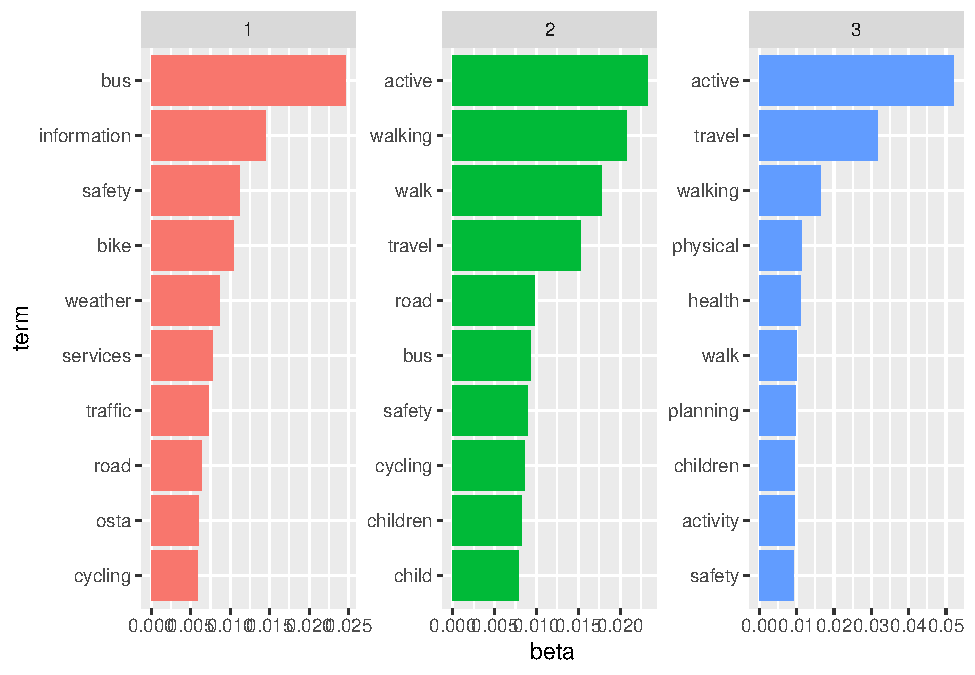
\includegraphics[width=1\linewidth]{AST-Framing-Ontario_files/figure-latex/policy-terms-1} \caption{\label{fig:policy-terms}Topics identified in the policy+practice corpus according to clusters of words. The per-word-per-topic probabilities are shown by beta.}\label{fig:policy-terms}
\end{figure}

\begin{figure}
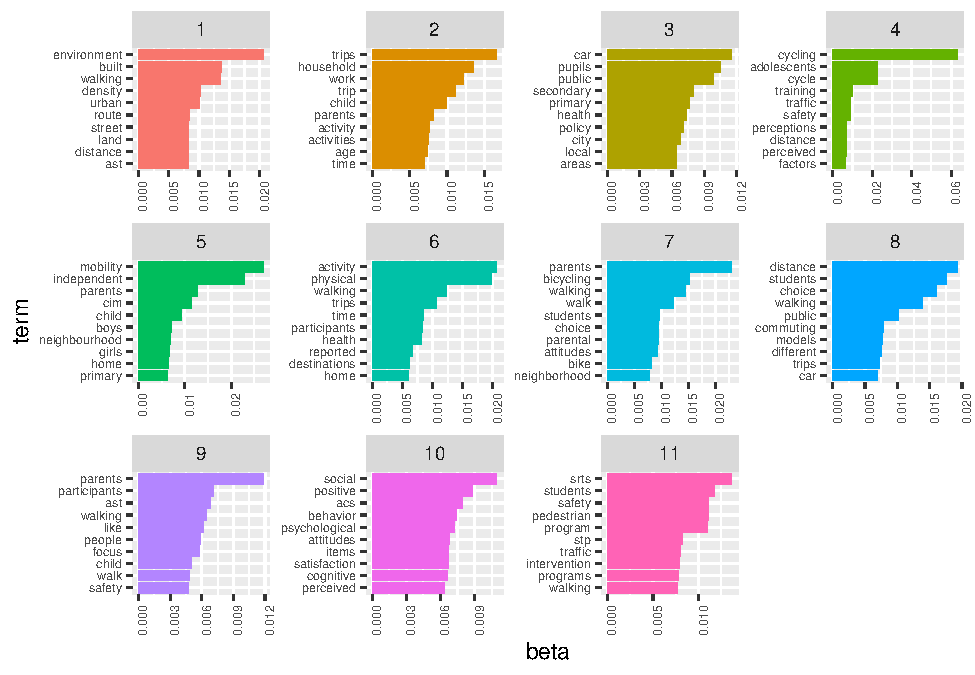
\includegraphics[width=1\linewidth]{AST-Framing-Ontario_files/figure-latex/academic-terms-1} \caption{\label{fig:academic-terms}Topics identified in the academic corpus according to clusters of words. The per-word-per-topic probabilities are shown by beta.}\label{fig:academic-terms}
\end{figure}

We conducted topic modelling to examine the different topics found in
the policy+practice and academic corpora. We estimated Latent Dirichlet
Allocation (LDA) models for each corpus. Parameter tuning suggests that
the policy+practice corpus has between 9 and 13 topics and the academic
corpus has between 17 and 25 topics. After running the LDA model for the
academic corpus, we realized the difficulty of interpreting as many as
17 topics based on the clusters of words that were identified. We
experimented with the model by adjusting the number of topics and
evaluating the output of terms in each topic. We found that there were 9
distinct topics that could be interpreted in the policy+practice corpus
and 11 topics in the academic corpus, after which there was too much
overlap for the clusters to be meaningfully interpreted. Figures
\ref{fig:policy-terms} and \ref{fig:academic-terms} present the main
terms that are associated with the topics found in each corpus.

In the policy+practice corpus, we identified the following topics based
on the cluster of words: (1) safety; (2) weather and busing; (3) active
travel planning; (4) walking; (5) resources for walking; (6) bicycling;
(7) active travel concerns; (8) benefits of active travel; and (9)
busing logistics. These topics indicate that STP stakeholder groups are
sending the message that walking and bicycling to school are healthy
travel modes for students, particularly in terms of physical activity.
We also found that information is shared to support parents and students
in using active modes to school, for example regarding the availability
of bicycling lanes and tips for route choice for walking.

The academic corpus has a higher number of topics likely due to the
volume of papers included. The following topics were identified based on
the clusters of words: (1) physical activity; (2) safe routes to school
for active travel; (3) behaviours and attitudes; (4) bicycling; (5)
walking; (6) built environment; (7) trip choice; (8) active school
travel interventions; (9) parents; (10) children's independent mobility;
and (11) public health and policies. This corpus reflects a broader
range of topics than the policy+practice corpus.

\hypertarget{frames}{%
\subsection{Frames}\label{frames}}

Based on the identified bigrams and topics, we determined that the
policy+practice corpus primarily frames AST as a health and
environmental issue. STP stakeholder groups appear to position walking,
bicycling, or rolling to school as beneficial to individual health, via
physical activity and improved mental health, and to the broader
community through a reduction in traffic and vehicle emissions. Here, we
present an example that illustrates how the health and environmental
frame is communicated:

\begin{quote}
\emph{Active school travel is a great way for children to be physically
active, which is associated with improved physical and mental health,
while making school zones safer, by reducing traffic volumes at and
around schools.}(Region of Leeds, Grenville and Lanark)
\end{quote}

Furthermore, we found that policy documents make claims about the
benefits of AST that are consistent with the findings of academic
research and evaluation.

\begin{quote}
\emph{There are lots of benefits in the classroom for children that walk
or cycle to school on a regular basis. Some of these benefits include
improved concentration and better coping with stress. Being outside
helps to prevent feelings of isolation and increases their social
interactions. Walking and biking to school can also save you money and
lead to fewer cars on the road.} (City of Ottawa)
\end{quote}

The secondary frame in policy documents is that AST is accessible and
feasible for children and parents. Despite the emphasis on the logistics
of busing in the topic modelling, the documents indicate that there is
an opportunity for or prospect of behaviour change. Some cities and
schools explain how children and parents can leave the car at home and
make the journey to school on foot or by bike. This frame encourages the
public to evaluate their own travel decisions and to access resources
(e.g., walking skills checklist) that will help them make AST a first
choice. Examples of this secondary frame include:

\begin{quote}
\emph{Help your students get started on the right foot - encourage them
to walk or bike to school when possible. Even leaving the car a block or
two and walking the rest of the way helps. It's good for the environment
and your health, and teaches your child independence and community
awareness.} (Halton District School Board)
\end{quote}

Finally, both AST frames present solutions to encourage AST. STP
stakeholder groups seem to be communicating that AST is a healthy and
easy option as a result of policy changes (e.g., available resources for
parents and children) and improvements to the built environment. This
could include examples of various efforts that are underway to support
AST including route planning.

\begin{quote}
\emph{School Travel Planning is a community-based approach that aims to
increase the number of students and adults choosing active and
sustainable travel to get to and from school. This approach addresses
concerns about safety, physical activity, and the environment.} (City of
Hamilton)
\end{quote}

\hypertarget{discussion}{%
\section{Discussion}\label{discussion}}

\hypertarget{current-ast-frames-in-ontario}{%
\subsection{Current AST frames in
Ontario}\label{current-ast-frames-in-ontario}}

Interpretation of the text assisted by natural language processing
reveals that AST in Ontario is primarily framed to parents as beneficial
to the health and wellbeing of children and to environmental
sustainability. The policy documents reflect the evidence that AST
contributes positively to children's physical health
\citep[see][]{faulknerActiveSchoolTransport2009, schoeppeAssociationsChildrenActive2015},
although the statements regarding the benefits of AST to children's
school performance are less well-supported in the extant literature
\citep{westmanTravelChildWellbeing2020}. STP stakeholder groups also
communicate that increasing AST may reduce traffic near and around
schools. This is conveyed presumably to alleviate parental concerns
about traffic and safety
\citep{eversParentSafetyPerceptions2014, mammenUnderstandingDriveEscort2012, rothmanAssociationsParentsPerception2015, wilsonUnderstandingChildParent2018}
or to reduce the frequency of risky behaviours from drivers around
schools \citep{rothmanSchoolEnvironmentStudent2017}.

In the secondary frame, AST is presented as an accessible and feasible
way for children to travel to and from school. Children and parents are
encouraged to adopt new travel behaviours. STP stakeholder groups
identified different ways that parents could encourage or support their
children to commute to school by using active modes (e.g., walking tip
sheets, walking school buses, etc.). The general emphasis of this frame
is communicating information that could change parental perceptions
about the ease of their children using active modes to school, which may
be seen by STP stakeholder groups as a ``modifiable'' factor
\citep[see][]{riaziCorrelatesChildrenIndependent2019}. In turn, this
could encourage parents to modify their routines and incorporate
opportunities for their children to use active modes to school.

Both frames present the AST issue in a positive light. Neither frame
appears to explain why declining rates of AST are a problem or convey
any urgency to this issue so that it attracts the attention of parents,
the general public, or policy makers. Communicating the potential
outcomes of increased AST may be persuasive arguments to motivate
behaviour change, but these frames do not seem to encourage parents or
the general public to view their current behaviour as problematic or
unhealthy for their children's development and their community. Thus,
behaviour change is presented as an option for some but not an
imperative for all. For example, parents who drive their children to
school have reported concerns about traffic volume around schools
\citep{mammenUnderstandingDriveEscort2012}, but may not recognize that
their own behaviour contributes to the problem that is perceived to
prevent their child from safely walking or bicycling to school
\citep{collinsSafeJourneysEnterprising2001}. Reynard et al.
\citeyearpar{reynardGrowthResilienceHow2021} similarly found in their
analysis of Canadian municipal documents that one of the dominant frames
presented the adoption of behaviours to help mitigate the climate crisis
as a choice but not ``the expected norm''.

We found that the proposed solutions in the secondary frame to increase
AST align with different levels of the SEM: 1) behaviour change from
households making different travel decisions; 2) policies that create
resources for AST; and 3) engineering solutions like bicycle lanes. This
reflects findings from the AST literature that a range of solutions are
needed to address different factors that influence AST
\citep[\emph{inter alia,
see}][]{mitraIndependentMobilityMode2013, panterAttitudesSocialSupport2010}.
The recognition of engineering changes may reflect the strong engagement
of engineering staff and municipal representatives in the Canadian STP
process
\citep{buttazzoniSupportingActiveSchool2018, mammenPuttingSchoolTravel2015},
as well as the evidence that the built environment influences mode
choice to school. However, it is beyond the scope of this paper to
assess whether the proposed solutions are perceived to be sufficient by
parents for increasing AST.

\hypertarget{implications-for-school-travel-planning}{%
\subsection{Implications for school travel
planning}\label{implications-for-school-travel-planning}}

STP stakeholders should problematize the significant decline in AST that
has occurred over recent decades in Canada and emphasize that this issue
merits urgent behaviour change. A negative framing that challenges the
social norm of driving could be more motivational to shift transport
modes, which would be consistent with other findings
\citep[see][]{waygoodCO2ValenceFraming2018}. Policy documents should
make it clear that continued use of nonactive modes to school can
deprive children of opportunities to increase physical activity and to
gain health and social benefits.

There is a noticeable lack of focus on certain household determinants of
AST in the two frames that needs to be addressed. For example, the role
of convenience and inclement weather in shaping household travel
decisions \citep{buliungSchoolTravelPlanning2011} and the complexity of
travel arrangements that must be coordinated by households
\citep[see][]{buliungLivingJourneySchool2021} were not found to be
discussed. The desire to escort children to school, which has been noted
by parents as a reason to continue driving
\citep{westmanWhatDrivesThem2017}, is also not adequately addressed by
STP stakeholders. Parental assessment of a child's ability to undertake
the journey to school was likewise overlooked despite its role in
decision making for mode choice to school
\citep{faulknerWhatQuickestEasiest2010}. Framing AST as a developmental
opportunity or a rite of passage that children have been denied could
challenge the prevailing culture of risk avoidance which discourages
parents from letting their children use active modes to school.

Future research and evaluation by STP stakeholders should investigate
how parents or the general public respond to messages or information
that encourages the adoption of AST and evaluate which are most
effective. It would be helpful to understand which frames would most
encourage behaviour change or increase political support for
interventions that address barriers to AST. This type of information
could ensure that educational strategies and promotional materials
increase buy-in for their target audience. If Canadian STP stakeholders
wish to involve more local residents in their efforts
\citep{buttazzoniSupportingActiveSchool2018}, it would also be
worthwhile for them to produce different materials that communicate why
this issue is important to the general public, regardless of whether
they currently have children commuting to/from school.

\hypertarget{limitations}{%
\subsection{Limitations}\label{limitations}}

A limitation of this study is that we only analyzed English-language
texts that were easily accessible to the general public on the websites
of STP stakeholders in Ontario. We did not include French-language
materials from Ontario's 12 French school boards (a mixture of public
and Catholic schools). Parents likely receive information about AST
directly from schools, which may contain more content that reflects the
local barriers to AST, but these materials were not used in our
analysis.

\hypertarget{conclusion}{%
\section{Conclusion}\label{conclusion}}

In this paper we examined how AST is framed in Ontario. Our analysis was
supported by the use of natural language processing techniques, and
reavealed that STP stakeholders frame AST as an accessible and feasible
way to travel to school that is valuable to children's health and to the
environment. STP stakeholders are communicating that this issue can be
addressed through household behaviour change and policy solutions.
Policy documents reveal that STP stakeholders are focusing on
``modifiable factors'' such as parental perceptions or micro-scale
elements in the built environment to increase rates of AST. However, AST
may not be framed sufficiently as a ``problem'' that requires urgent
intervention, which may impact how parents respond to behaviour change
initiatives and limit awareness in the general public. In their public
materials about AST, STP stakeholders should emphasize why AST rates
should increase in local communities and how the negative effects of
nonactive modes to school may impact children's health and wellbeing.

\renewcommand\refname{References}
\bibliography{bibliography.bib}


\end{document}
